% !TEX root = thesis-thomas-tiotto.tex

\section{Explaining the Most Probable Explanation} \label{sec:explaining-the-most-probable-explanation}
The paper \enquote{Explaining the Most Probable Explanation} by \cite{Butz2018} inserts itself into the literature concerned with the explainability of Bayesian Networks.
In particular, taking \cite{lacave2002review}'s classification presented in Sec. \ref{sec:explainability-in-bayesian-networks}, it attempts to define a \textit{verbal explanation} to the \textit{knowledge base} and of the \textit{propagated evidence}.
Unlike \cite{lacave2002review}'s definition of explanation of a knowledge base and of other previous works, the paper is not concerned with finding the most probable assignment of variables that would explain the given evidence but, rather, the inverse problem.
By starting with evidence and finding a maximally probable configuration, the authors hope \enquote{to look at the complete scenario to get an overview before deciding which variables should be focused on}; that is, the goal appears to give the user an overview of the situation.  

The initial claim of the paper is that even though BNs provide a graphical structure to the knowledge base, they remain of difficult interpretation for domain experts.
The examples brought to justify the claim are that edges in the graph do not necessarily represent causal dependencies and that d-separation (defined in \ref{subsec:d-separation}) may be confusing.
The authors plan to address this claim by constructing a \textit{dialogue} with the user and thus to continue in the long tradition of dialogical approaches to explaining BNs.

The defining characteristic of their approach is that the domain expert is able to \enquote{argue} with the MPE and investigate alternative explanations.
The complete methodology, that is executed over three steps, is shown in Fig. \ref{fig:butz-methodology}.
The first step is the construction of the \enquote{knowledge base}, which is nothing else than a probability tree representing a \enquote{chain of deduction} constructed following the strongest probabilistic dependencies between variables in the BN.
Such a knowledge base is convenient because the document plan for the Natural Language Generation step is directly derived from it.
One issue that is immediately apparent is that this greedy approach does not \enquote{generate the MPE solution} as the authors claim, as noted in Subsec. \ref{subsec:bnupdating}.
This does not discredit the argumentative method as a whole, as it is not necessary for the user to be arguing the MPE to derive a good explanation; this ties into one of the main findings in the previous sections that many xAI researchers are only focusing on half of what an explanation is.
A good explanation is not given only by its formal properties but, most importantly, by how it acts as an interface between the real \textit{user} and the model.
This is what \cite{abdul2018trends} mean when they lament that \enquote{despite their mathematical rigor, these works \textit{[referring to the existing explainability methods]} suffer from a lack of usability, practical interpretability and efficacy on real users.}

\begin{figure}[htbp]
\centerline{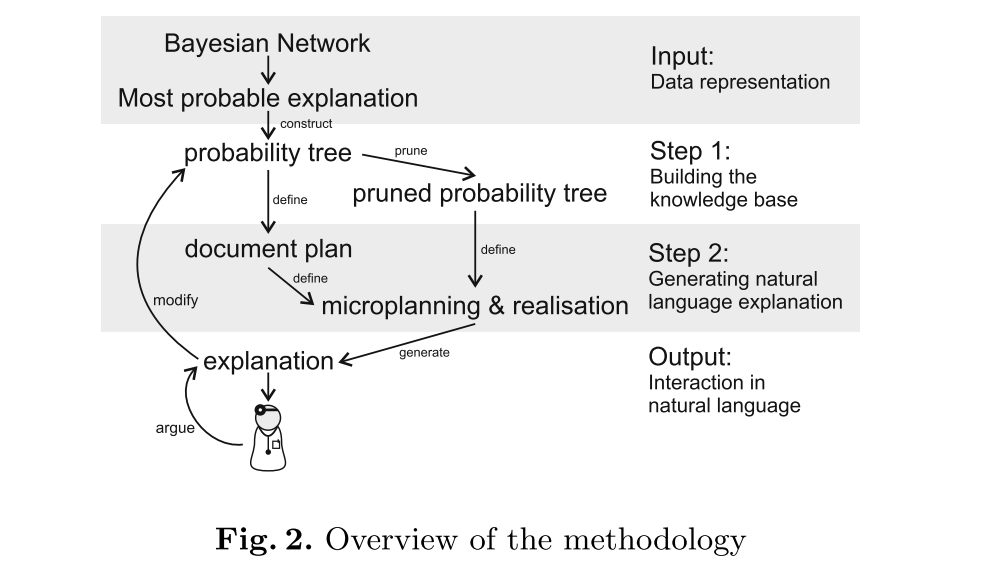
\includegraphics[width=\columnwidth]{literature-review/images/butz-methodology}}
\caption{\cite{Butz2018}}
\label{fig:butz-methodology}
\end{figure}

The document plan for the argumentation follows the same chain of strongest dependencies constructed in the knowledge base until the expert disagrees; at that point, the user is presented with an alternative \enquote{MPE}.
An example of how the document plan may look after interaction with the user is shown in Fig. \ref{fig:butz-tree}.
All the natural language phrasing is generated via boilerplates that realise both the micro-planning phase and the generation of the text.

\begin{figure}[htbp]
\centerline{
\includegraphics[width=\columnwidth]{literature-review/images/butz-tree}}
\caption{\cite{Butz2018}}
\label{fig:butz-tree}
\end{figure}

The authors recognise that such chains of deduction could become long and cognitively overloading in the case of larger BNs, as every variable in the tree is explained by all its ancestors.
A solution they propose is that of \textit{pruning} the probability tree by excluding d-separated nodes and those under a certain threshold of significance.
They also adapt some methods from literature to perform \textit{conflict analysis}; that is, only variables that contribute positively to the explanation are maintained in the document plan.

On the whole, the paper offers a compelling explanation method for BNs by building on an established tradition of explainability through dialogue.
The work, though, takes some methodological missteps and also continues the \enquote{sin} of not validating its claims on real users, that is one of the primary gaps in the xAI field that were identified in the previous sections.
